\section{Test-beam Setup and Experimental Apparatus }
\label{sec:tbeam}

We performed the measurements at the T9 beam-line of the CERN East-Area test-beam facility and 
the H2 beam-line of the CERN North-Area test-beam facility. The T9 beam-line provides secondary 
beams of energies ranging between $0.5$~GeV and $10$~GeV based on the primary proton beam source 
from the Proton Synchrotron (PS), while the H2 beam-line provides secondary beams of energies 
ranging between $20$~GeV and $400$~GeV based on the primary proton beam source from the Super 
Proton Synchrotron (SPS). The beams are composed of 
a mixture of electrons and pions. The electron fraction in the beam at H2 is typically larger than 75\%
while at T9 it is typically about 10\%. 

Trigger counters made of photo-multipliers coupled to $4$~$\mathrm{cm}$~$\times$~$4$~$\mathrm{cm}$ 
plastic scintillators are used 
to initiate the read out of the data acquisition (DAQ) system. The DAQ system
uses a CAEN V1742 switched capacitor digitizer based on the DRS4 chip~\cite{DRS4}. Wire chambers
are used to measure the position of each incident beam particle in the plane transverse
to the beam-line. A stack of lead or tungsten absorbers of different thicknesses are 
placed about $5$~mm in front of the CdTe sensor, which is 
enclosed within a copper box. The signals from the CdTe sensor are amplified using 
using a Hamamatsu C5594 amplifier~\cite{HamaAmpDataSheet} with a bandwidth of
$1.5$~GHz and providing a voltage gain of $36$~dB. A $10$~dB attenuator was used to attenuate the input signal 
to the amplifier for beam energies of 50 GeV and above to adjust the CdTe signal to the dynamic range of the amplifier. 
A micro-channel plate photo-multiplier (MCP-PMT)
detector is used to provide a very precise reference time-stamp. At the T9 beam-line,
a Hamamatsu R3809U MCP-PMT~\cite{HamaMCPDataSheet} is placed just upstream of the absorber material. 
At the H2 beam-line a Photek 240 MCP-PMT~\cite{PhotekDataSheet} is used, which contains a significant 
amount of absorber material (about 1.8 radiation lengths), and is therefore placed 
just downstream of the CdTe sensor to avoid inducing an early electromagnetic shower.
The precision of the time measurement for both types of MCP-PMTs is less than 
$10$~ps~\cite{MCPShowerMaxPaper,Anderson:2015gha}. As the purity of the electron beam at the T9 beam-line is
significantly lower than at the H2 beam-line, we use a LYSO crystal
optically coupled to an MCP-PMT as a means of discriminating the electrons from the pions
in the beam. The LYSO cube is about 1.7cm thick, corresponding to 1.5 radiation lengths, 
and is placed close to the shower maximum. Therefore, electron particles will produce 
electromagnetic shower particles which create scintillation light in the LYSO crystal, 
while pions do not. The efficiency for identifying electrons with this method was 
cross checked using a Cherenkov counter and was observed to be greater than $95\%$.
The entire setup of absorber, reference counter and CdTe sensor box is housed in an aluminum
box to provide further shielding against environmental noise.
The schematic diagrams of the experimental setups at H2 and T9 
are shown in Figure~\ref{fig:BeamSchematicDiagram}, and a photograph
of the contents of the aluminum box for the setup at T9 is shown in 
Figure~\ref{fig:SetupPhoto}.


%Fig: Diagram of detector elements
\begin{figure}[htbp] 
\centering
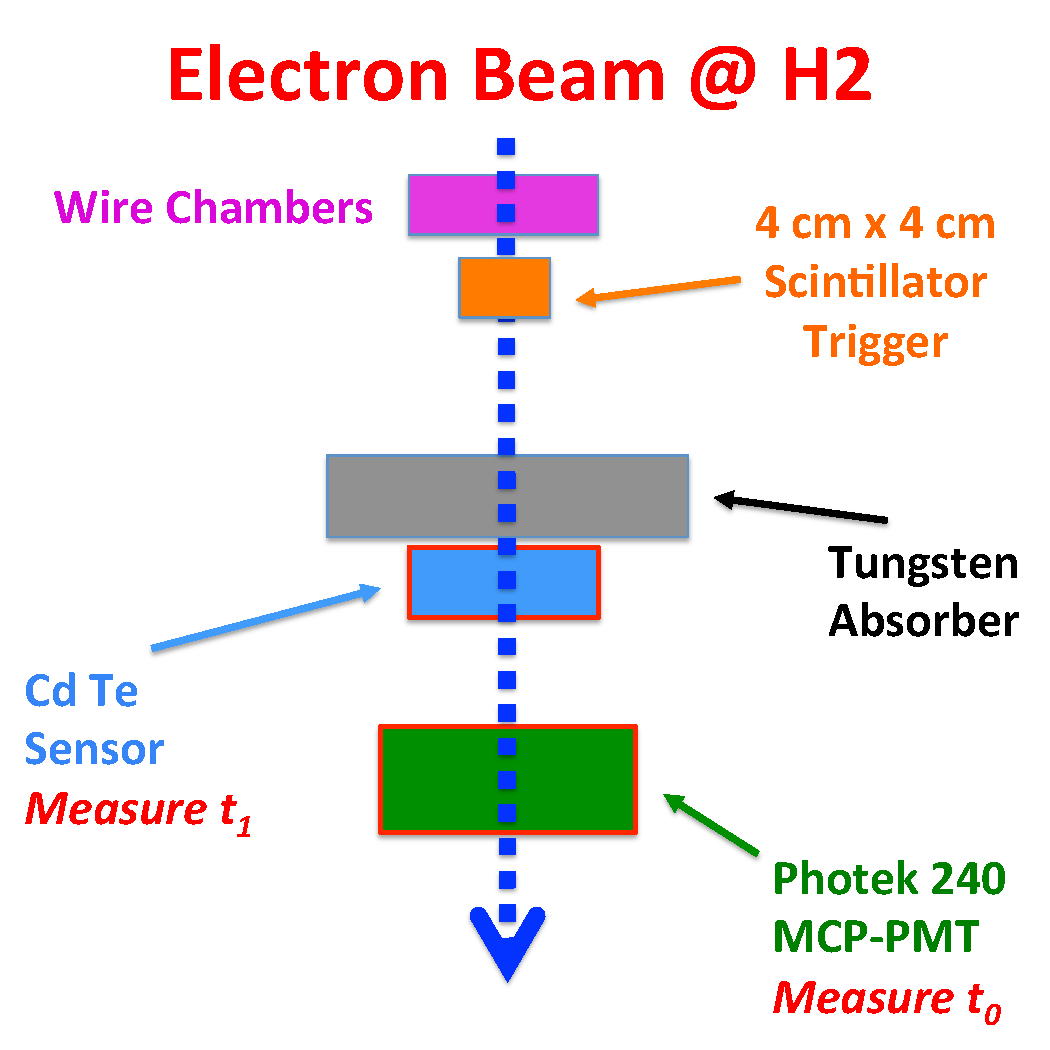
\includegraphics[width=0.49\textwidth]{figures/H2_BeamSchematicDiagram.pdf} 
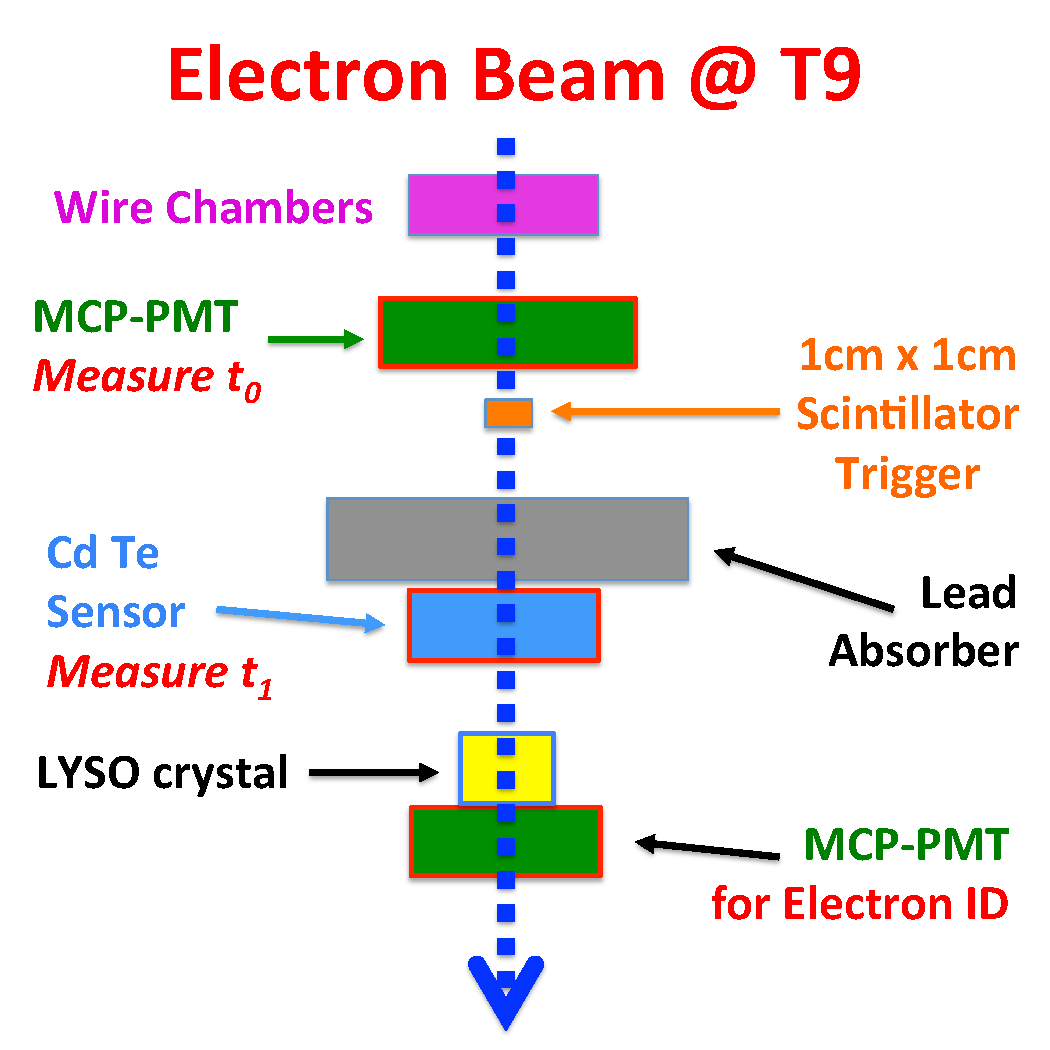
\includegraphics[width=0.49\textwidth]{figures/T9_BeamSchematicDiagram.pdf} 
\caption{Schematic diagrams of the test-beam setups at H2 (left) and T9 (right) are shown. 
The time-stamps $t_0$ and $t_1$ are defined in Section~\ref{sec:reco}.} 
\label{fig:BeamSchematicDiagram} 
\end{figure} 

\begin{figure}[htbp] 
\centering
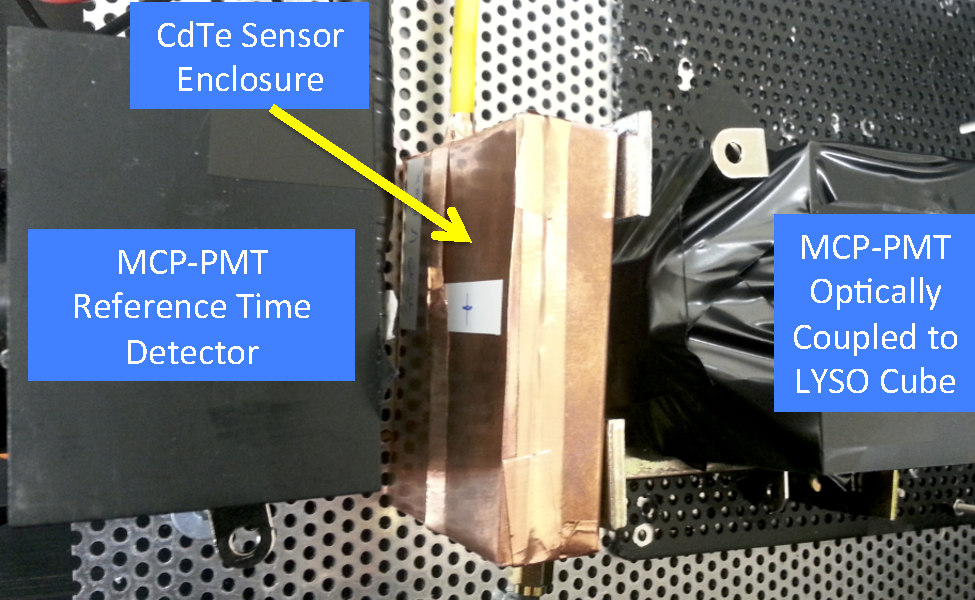
\includegraphics[width=0.75\textwidth]{figures/T9SetupPhoto.pdf} 
\caption{ Photograph of the setup used in the T9 beam line. The reference timing MCP-PMT 
is located on the leftmost region of the photo, followed to the right by a scintillator counter, 
the copper box enclosing the CdTe sensor and an MCP-PMT optically coupled to a LYSO cube. 
The lead absorber is not present in the photo and was later inserted in front of the copper box.} 
\label{fig:SetupPhoto} 
\end{figure} 


The horizontal and vertical position measurements from the wire chamber are used to determine the location
of the CdTe sensor relative to the beam and to align the beam. In 
Figure~\ref{fig:BeamSensorPosition}, we show the average amplitude measured in the
CdTe sensor after $6$~radiation lengths of tungsten absorber
as a function of the horizontal and vertical positions as measured by the wire chamber. Based
on these plots, we can restrict our measurements to those electrons whose impact points are close
to the center of the CdTe sensor.

%Fig: Beam profile X-Y plot
\begin{figure}[htbp] 
\centering
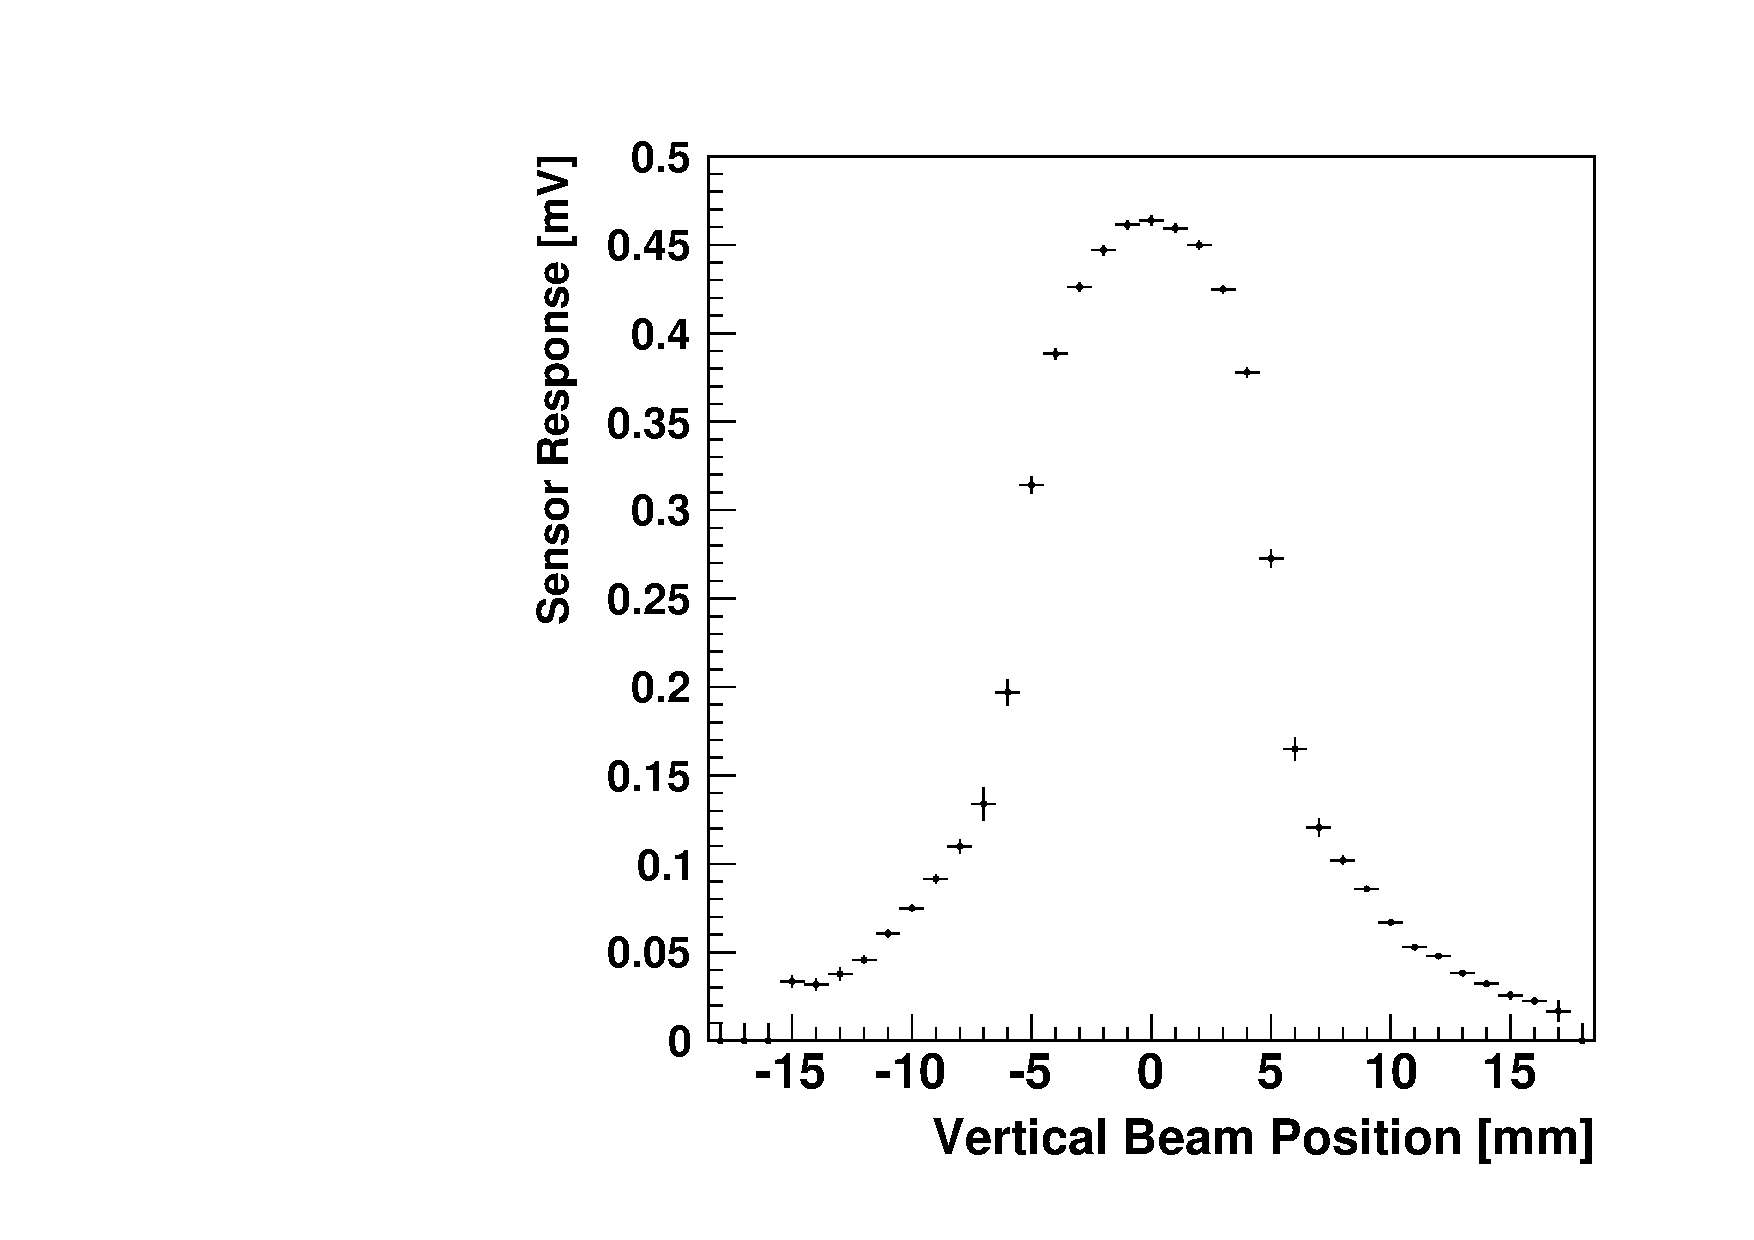
\includegraphics[width=0.49\textwidth]{figures/CdTeProfile_X.pdf} 
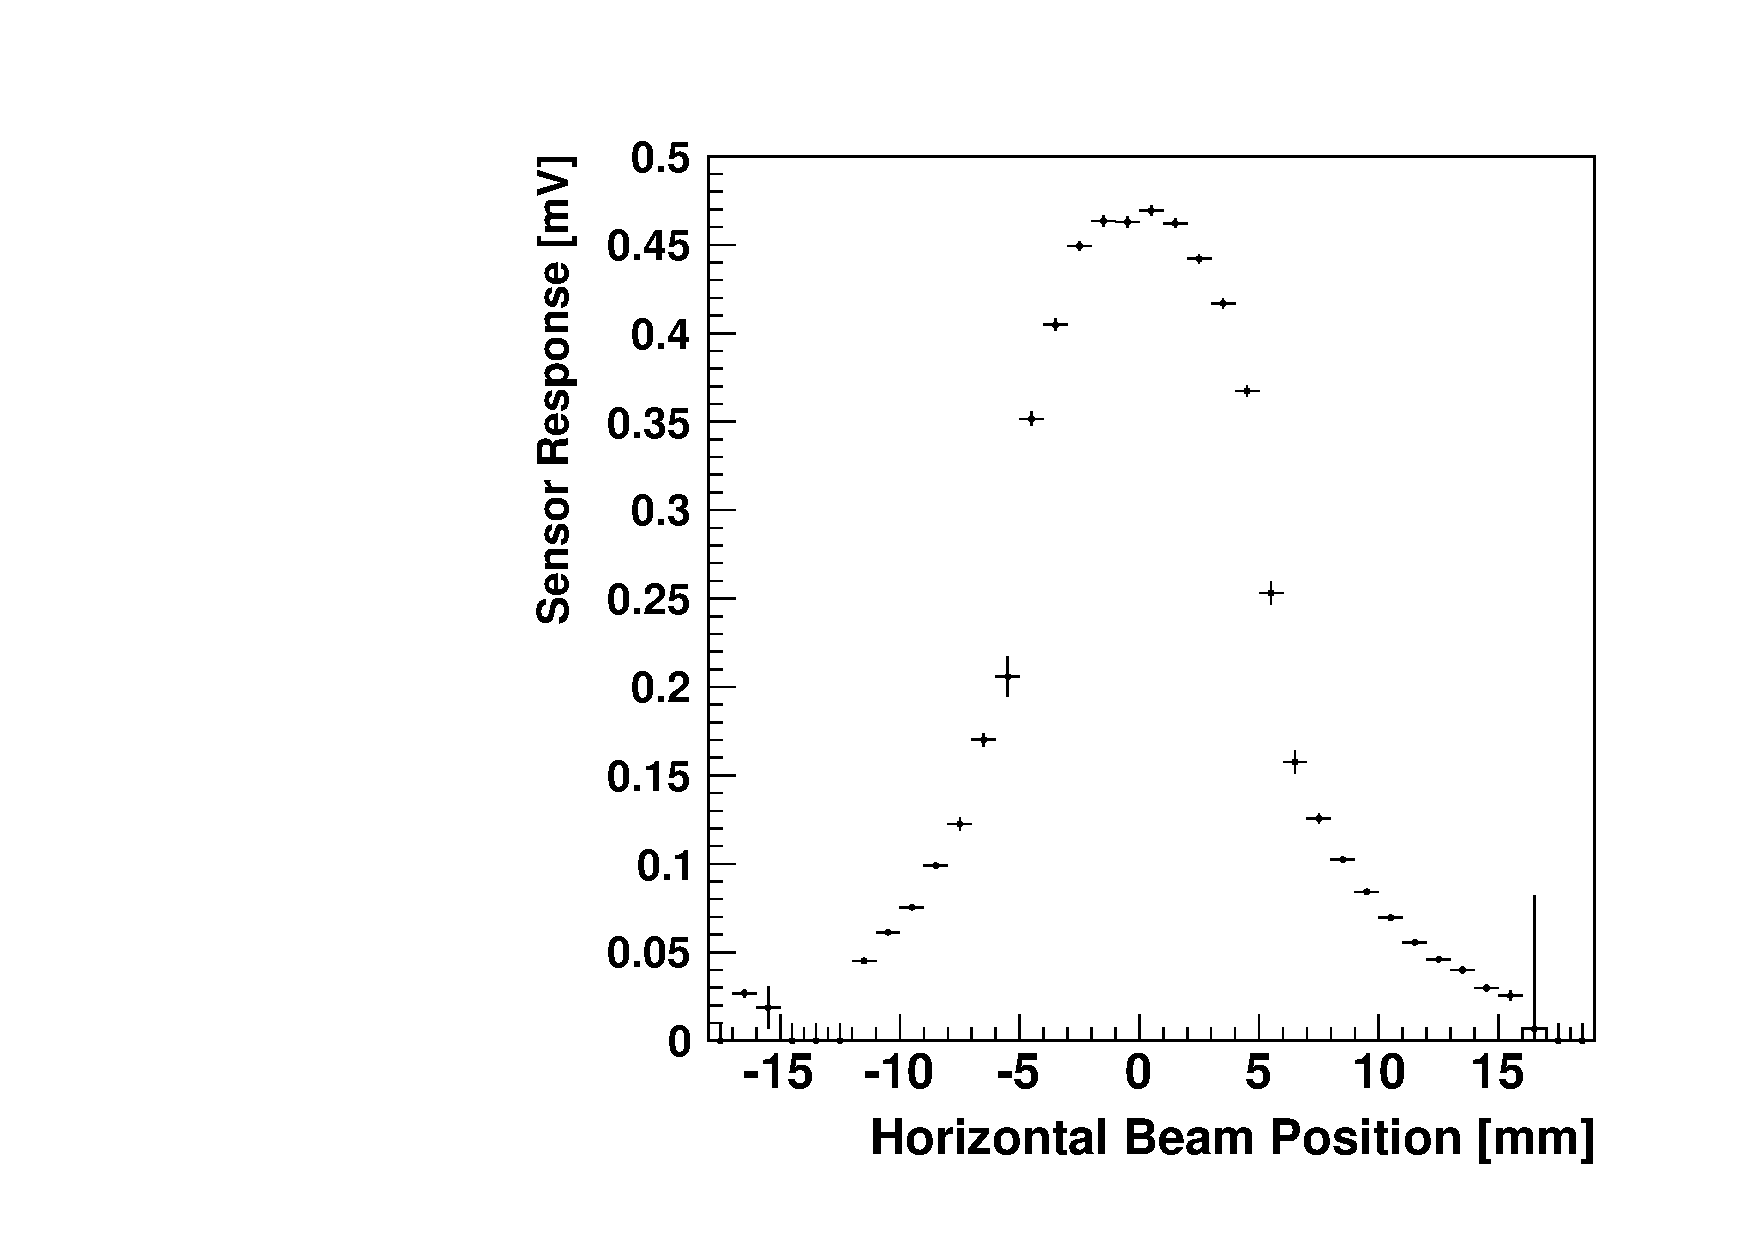
\includegraphics[width=0.49\textwidth]{figures/CdTeProfile_Y.pdf} 
\caption{The average amplitude measured in the CdTe sensor is plotted as a function of 
the horizontal and vertical positions of the beam particle as measured by the wire chamber. The measurement shown was performed with electrons of 100 GeV and $6\, X_0$ of tungsten absorber.} 
\label{fig:BeamSensorPosition} 
\end{figure} 

